\subsection{Ba bước giải quyết bài toán}
\begin{frame}{Ba bước giải quyết bài toán}
  \textbf{Bước 1: Quan sát, phân tích thông tin và thiết lập mô hình (nếu cần)}
    \begin{itemize}
        \item Điều cần tìm là gì? Mối liên hệ nào chưa biết?
        \item Có những thông tin nào quan trọng? Những kiến thức nào có thể sử dụng?
        \item Dự đoán hiện tượng.
        \item Tìm cách biến chúng thành phương trình toán học, thiết lập mô hình (nếu cần).
        \item Những đại lượng nào liên quan? Có thể sử dụng phân tích thứ nguyên để dự đoán mối liên hệ không?
  \end{itemize}
\end{frame}

\begin{frame}{Ba bước giải quyết bài toán}
  \textbf{Bước 2: Xử lý bài toán}
    \begin{itemize}
        \item Khảo sát biểu đồ vật tự do.
        \item Dựa vào các thông tin có được (liên kết, định luật, định lý, xấp xỉ…) thiết lập số phương trình tương ứng với số ẩn.
        \item Giải toán.
    \end{itemize}
    \begin{figure}
        \centering
        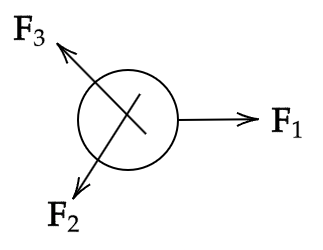
\includegraphics[width=0.25\textwidth]{Slides/Figure/fbd.png}
        \caption{Biểu đồ vật tự do}
    \end{figure}
\end{frame}

\begin{frame}{Ba bước giải quyết bài toán}
  \textbf{Bước 3: Kiểm tra và đánh giá}
    \begin{itemize}
        \item Kiểm tra thứ nguyên của kết quả.
        \item Đối chiếu với các trường hợp đặc biệt, giới hạn.
        \item Quá trình làm có sai sót không? Mô hình lựa chọn có đáng tin cậy không?
        \item Cách tiếp cận cho bài toán là đặc biệt và duy nhất hay có thể đáp ứng cho một loạt các bài toán khác?
        \item Nhận xét ý nghĩa vật lý của lời giải và thử lý giải một cách trực giác.
    \end{itemize}
\end{frame}

\subsection{Ví dụ 1}
\begin{frame}{Ví dụ 1}
Trên một cái nêm khối lượng \(M\) có góc nghiêng \(\alpha\) so với mặt đất đặt một vật có khối lượng \(m\). Hệ số ma sát giữa vật và nêm là \(\mu_1\), giữa nêm và mặt đất là \(\mu_2\). Tìm gia tốc của vật và nêm.
\begin{figure}
    \centering
    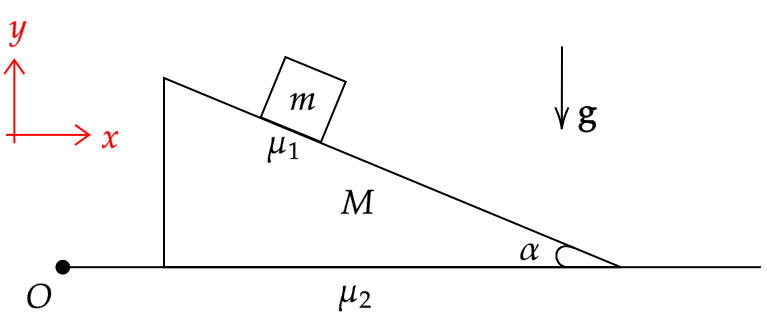
\includegraphics[width=0.5\textwidth]{Slides/Figure/wedgemass.png}
    \caption{Hệ nêm và vật}
\end{figure}
\end{frame}

\begin{frame}{Ví dụ 1}
\begin{columns}
    \begin{column}{0.5\textwidth}
\textbf{Bước 1: Lựa chọn hệ tọa độ phù hợp, phân tích lực.}
\end{column}
    \begin{column}{0.5\textwidth}
\begin{figure}
    \centering
    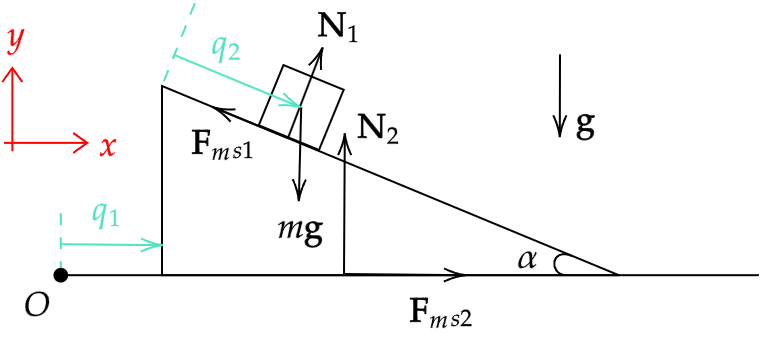
\includegraphics[width=0.8\textwidth]{Slides/Figure/wedgemass1.png}
\end{figure}
\end{column}
\end{columns}
\textbf{Bước 2: Thiết lập hệ 6 phương trình 6 ẩn \(N_1\), \(N_2\), \(F_{ms1}\), \(F_{ms2}\), \(q_1\), \(q_2\).}
\scriptsize
\begin{columns}
\begin{column}{0.4\textwidth}
\begin{align*}
    \begin{cases}
        \mathbf{F_{ms1}}+\mathbf{N_1}+m\mathbf{g}=m\mathbf{a_1} \\
        -F_{ms1}+mg\sin\alpha=m (\ddot q_2+\ddot q_1\cos\alpha) \\
        N_1-mg\cos\alpha=m\ddot q_1\sin\alpha
    \end{cases}
\end{align*}
\end{column}
\begin{column}{0.3\textwidth}
\begin{align*}
    \begin{cases}
        -\mathbf{N_1}-\mathbf{F_{ms1}}+\mathbf{N_2}+\mathbf{F_{ms2}}+M\mathbf{g}=M\mathbf{a_2}\\
        -N_1\cos\alpha-F_{ms1}\sin\alpha+N_2-Mg=0\\
        -N_1\sin\alpha+F_{ms1}\cos\alpha+F_{ms2}=M\ddot{q_1}
    \end{cases}
\end{align*}
\end{column}
\begin{column}{0.3\textwidth}
\begin{align*}
    \begin{cases}
        F_{ms1}=\mu_1 N_1 \\
        F_{ms2}=\mu_2 N_2
    \end{cases}
\end{align*}
\end{column}
\end{columns}
\normalsize
\end{frame}

\begin{frame}{Ví dụ 1}
    Giải hệ phương trình trên ta được:
    \begin{equation*}
    \ddot q_1 =
g \frac{ 
M\mu_2 + m\Big[(\mu_1+\mu_2)\cos^2\alpha + (\mu_1\mu_2-1)\sin\alpha\cos\alpha\Big]}
{ M - m\Big[(\mu_1\mu_2-1)\sin^2\alpha + (\mu_1+\mu_2)\sin\alpha\cos\alpha\Big] },
\end{equation*}
    \begin{equation*}
        \ddot q_2 =
g  
\frac{ M\Big[ (1-\mu_1\mu_2)\sin\alpha - (\mu_1+\mu_2)\cos\alpha \Big]
+ m\Big[ \sin\alpha - \mu_1\mu_2\sin^2\alpha - (\mu_1+\mu_2)\cos\alpha \Big]}
{ M - m\Big[ (\mu_1\mu_2-1)\sin^2\alpha + (\mu_1+\mu_2)\sin\alpha\cos\alpha \Big]}.
    \end{equation*}
\textbf{Bước 3: Kiểm tra và đánh giá}
\begin{itemize}
    \item Kiểm tra thứ nguyên: \([ML^2T^{-2}]\) của gia tốc.
    \item Việc gọi ra các lực liên kết như \(N_1\), \(N_2\) có thể áp dụng cho nhiều bài toán khác.
\end{itemize}
\end{frame}

\subsection{Ví dụ 2}
\begin{frame}{Ví dụ 2}
    Một quả cầu có khối lượng \(m\), thể tích \(V\) được nhúng trong một chất lỏng có khối lượng riêng \(\rho\). Khi di chuyển ở trong chất lỏng, vật chiu một lực cản nhớt \(\mathbf F_c=-k\mathbf v\). Biết rằng ban đầu vật xuất phát tại gốc tọa độ với vận tốc \(\mathbf v_0\) theo phương x. Tìm tọa độ của vật theo thời gian. Coi \(v_0\) là đủ nhỏ để hợp lực gây bởi áp suất tác dụng lên vật gần đúng bằng lực đẩy Archimedes.
\begin{figure}
    \centering
    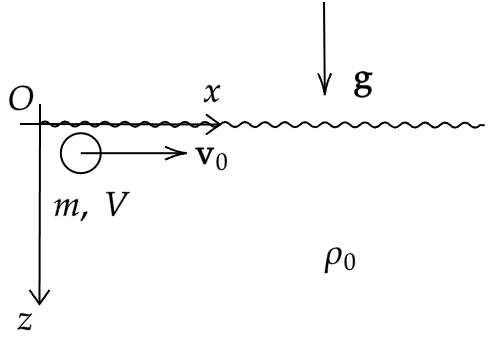
\includegraphics[width=0.4\textwidth]{Slides/Figure/masatnhot.png}
\end{figure}
\end{frame}

\begin{frame}{Ví dụ 2}
\begin{columns}
    \begin{column}{0.5\textwidth}
\textbf{Bước 1: Phân tích lực.}
\end{column}
    \begin{column}{0.5\textwidth}  
\begin{figure}
    \centering
    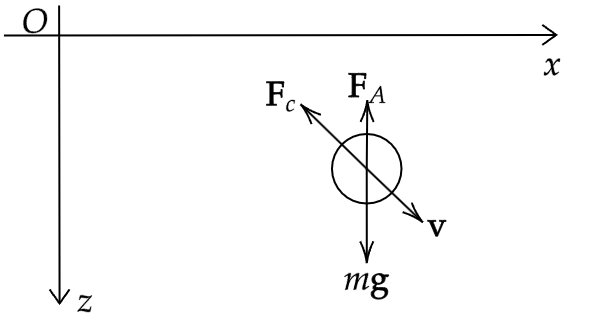
\includegraphics[width=0.7\textwidth]{Slides/Figure/masatnhot1.png}
\end{figure}
\end{column}
\end{columns}
\textbf{Bước 2: Thiết lập hệ phương trình 2 ẩn \(x\), \(y\) từ \(m\mathbf a=\mathbf F_c+\mathbf F_A+m\mathbf g\).}
\scriptsize
\begin{columns}
\begin{column}{0.5\textwidth}
\begin{align*}
    \text{Phương x:}\quad
    \begin{cases}
    m\ddot{x} = -k\dot{x}. \\
    m\int_{v_0}^{\dot{x}} \dfrac{d\dot x}{\dot x} = -k\int_0^t dt. \\
    \dot x=v_0 \exp(\dfrac{-kt}{m}).
    \end{cases}
\end{align*}
\end{column}
\begin{column}{0.5\textwidth}
\begin{align*}
    \text{Phương z:}\quad
    \begin{cases}    
    m\ddot{z} = -\rho g V + mg - k\dot{z}. \\
    m\int_{0}^{\dot z} \dfrac{d(k\dot z+\rho g V-mg)}{k\dot z+\rho g V-mg} =-k\int_0^t dt.\\
    \dot{z} = \left(\dfrac{mg - \rho g V}{k}\right)\left[1 - \exp\left(-\frac{k t}{m}\right)\right].
    \end{cases}
\end{align*}
\end{column}
\end{columns}
\normalsize
\end{frame}

\begin{frame}{Ví dụ 2}
Tích phân theo thời gian 2 phương tình trên:
\begin{equation*}
    x(t) = \dfrac{m}{k}v_0\left(1 - \exp\left(-\dfrac{kt}{m}\right)\right).
\end{equation*}
\begin{equation*}
    z(t) = \dfrac{mg - \rho g V}{k}t - \dfrac{m}{k}\left(\dfrac{mg - \rho g V}{k}\right)\left[1 - \exp\left(-\dfrac{kt}{m}\right)\right].
\end{equation*}
\textbf{Bước 3: Kiểm tra và đánh giá}
\begin{itemize}
    \item Kiểm tra thứ nguyên: \([L]\) của tọa độ.
    \item Khi \(m\to\infty\) hoặc \(k\to 0\), từ khai triển Taylor: \(x(t)\approx v_0 t\) và \(z(t)\approx \frac12 g t^2\).
    \item Khi trọng lực bằng lực đẩy Archimedes: \(z(t)=0\).
\end{itemize}
\end{frame}